
The goal of our fast path is to forgo the overhead associated with 
communicating with 
the TM to begin and commit transactions. This is particularly important for short transactions, where the begin and commit overhead is not amortized
across many operations.
We therefore focus on single-key transactions.

To this end, we introduce in Section~\ref{ssec:fast-api} a streamlined  \emph{fast path (FP)}
API that jointly executes multiple API calls of the original TPS.
We proceed, in Section~\ref{ssec:fast-algorithm}, to explain a high-level general fast path algorithm 
{for any system that follows the generic schema of  Algorithm~\ref{alg:schema} above}. 
Finally, in Section~\ref{ssec:fast-impl}, we describe our implementation of the fast path in \sys, and 
important practical optimizations we applied in this context.
 
\subsection{API}
\label{ssec:fast-api}

%\paragraph{API.}
For brevity, we refer to the TPS's API calls  begin, read, write, and commit as \code{b, r, w}, and \code{c} respectively, and 
we combine them to allow fast processing.
The basic FP transactions are singletons, i.e., transactions that perform a single
read or write. These are supported by the APIs: 
\begin{description}
\item[brc(key)] -- begins an FP transaction, reads key within it, and commits.
\item[bwc(key,val)] -- begins an FP transaction,  writes val into a new version of key that exceeds all existing ones, and commits.
\end{description}

We further support a fast path transaction consisting of a read and a dependent write, via a pair of API calls:
\begin{description}
\item[br(key)] -- begins an FP transaction and  reads the latest version of key. 
Returns the read value along with a version ver.
\item[wc(ver, key,val)] -- 	validates that key has not been written since the  \code{br} call that returned ver, writes val into a new version of key, and commits.
\end{description}

Read-only transactions never abort, but \code{bwc} and \code{wc} may abort. 
If an FP transaction aborts, it can be retried either via the fast path again, or as a regular transaction.

\remove{
We note that though the FP API richness can potentially complicate development, this drawback may be abstracted 
away by high-level access semantics. For example, a SQL database (e.g., Phoenix~\cite{Phoenix})
can select the most appropriate API in its query optimizer, transparently to the user.  
}

\remove{
A more elaborate example is a read-modify-write API: 
\begin{description}
\item[brwc(key,f)] -- begins an FP transaction,  reads the latest version of key, applies $f$ to it (on the server side), 
	writes the result into a new version of key that exceeds all existing ones, and commits.
\end{description}

To use the above API, the programmer has to encapsulate the transaction logic in a function for server-side processing. 
Alternatively, we allow FP transactions to unfold dynamically much like regular  transactions do.
A dynamic FP transaction may instead begin with a \code{br} call, perform client-side processing, and then call the following
function to update either the same or a different key: 

\begin{description}
\item[wc(key,val)] -- writes val into a new version of key that exceeds all existing ones, and commits.
\end{description}

Moreover, we do not restrict FP transactions to perform a single read -- any number of \code{r}'s may be called between the \code{br} 
and \code{wc}. The supported types of FP transactions are summarized in Table~\ref{table:fp-types}.
Note, however, that all calls must be directed at the same region, else the transaction is not local.
In case an FP transaction dynamically discovers that it needs to access additional regions, it is aborted and should be restarted as a regular transaction. 

\begin{table}[htb]
%\def\arraystretch{1.5}%  1 is the default, change whatever you need
\centerline{
\begin{tabular}{l  @{\hspace{2em}} l}
Call sequence & Transaction type\\
\hline
\code{br} & single read\\
\code{bwc} & single write\\
\code{br, r*} &  multi-read\\
\code{br, r*, wc} & multi-read, single write\\
\code{brwc} & server-side single-read-write\\
%\hline
\end{tabular}
}
\caption{Supported FP transaction types.}
\label{table:fp-types}
\end{table}

In principle, it would have been possible to also allow \code{w} calls in the span of an FP transaction, 
but in this case, it is not possible to forgo the two-phase execution. 
That is, the \code{w} calls would need to indicate write intents, and  to be atomically committed (or aborted) during the final \code{wc} 
(or \code{c}) call. 
Given the limited benefit and extra complexity of allowing many writes in FP transactions, we do not support this option in our solution.

}


\subsection{Generic fast path algorithm}
\label{ssec:fast-algorithm}



\begin{algorithm}[htb]
%\small
%\hspace{10mm}\\

\underline{Client-side logic:}
\begin{algorithmic}[1]
%\small
\Procedure{brc}{key} \label{l:brc}
\State rec  $\leftarrow$ ds.get(last committed record of key)  \Comment no preGet
\State  return rec.value
\EndProcedure
% \Statex
\Procedure{bwc}{key, value} 
%	\State old $\leftarrow$ ds.get(last version of key)
%	\If{old.commit = nil}  \Comment  tentative value -- abort 
%		\State return abort 
%	\EndIf
	\State return {ds.putVersion}($\infty$, key, value)
\EndProcedure
% \Statex
\Procedure{br}{key} 
\State rec  $\leftarrow$ ds.get(last committed record of key) \Comment no preGet
\State  return \tuple{rec.version, rec.value}
\EndProcedure
% \Statex
\Procedure{wc}{ver, key, value} 
\State return {ds.putVersion}(ver, key, value)
\EndProcedure
\Statex
\algstore{fp}
\end{algorithmic}

\underline{Data store (stored procedure) logic:}
\begin{algorithmic}[1]
\algrestore{fp}
%\small
\Procedure{putVersion}{old, key, value} 
\Statex \Comment used by FP writes (\code{bwc} and \code{wc})
%\Atomic 
	\If{key has no tentative version $\wedge$\\
		\hspace{7mm} last committed version of key $\le$ old}
		\State ver $\leftarrow$ F\&I(key's maxVersion) $+1$   \label{l:fi}
		\State ds.put(key, value, ver, ver) 	\Comment no prePut	%  \tuple{key, ver} with commit = ver  
		\State return commit
	\Else 
		\State return abort 
	\EndIf
%\EndAtomic
\EndProcedure

\Statex
\Procedure{preGet}{$ts_r$, key}   \label{l:txr}
\Statex \Comment executed atomically with ds.get call, once per key 
\State bump(key's maxVersion, $ts_r$)
%\State return get(key)
\EndProcedure
% \Statex
\Procedure{prePut}{key, val, $ts_r$, nil}   \label{l:txw}
 \Statex \Comment checked atomically before put (by transactional write)
 \If{key has a committed version that exceeds $ts_r$} 
 	\State abort 
 \EndIf
\EndProcedure

\Procedure{preUpdate}{key, \inred{$ts_r$}, commit, $ts_c$}   \label{l:txu}
\Statex \Comment executed atomically with ds.update call (by  post-commit) 
\State bump(key's maxVersion, $ts_c$)
\EndProcedure
\end{algorithmic}
\caption{Generic support for FP transactions; each data store operation is executed atomically.}
\label{alg:fp}
\end{algorithm}

The generic fast  path algorithm, which we present in Algorithm~\ref{alg:fp}, consists of two parts: 
client side-logic, and logic running within the underlying data store. 
The latter is implemented as a stored procedure, %%%%%%%%. 
Specifically, it supports a new flavor of put, \emph{putVersion}, which is used by singleton writes, 
and it extends the put, get, and update APIs used by regular transactions with additional logic.  
The new logic is presented in the \emph{preGet}, \emph{prePut}, and \emph{preUpdate} procedures, 
which are  executed before, and atomically with, the corresponding data store calls.

Singleton reads (line~\ref{l:brc}) simply return the value associated with the  latest committed version of the requested key they encounter.  
They ignore tentative versions, which may lead to missing the latest commit in case its post-commit did not complete, 
but is allowed by our semantics. 
FP reads can forgo the begin call since they do not need to obtain a snapshot time a priori. 
They can also forgo the commit call, since they perform a single read, and hence their `snapshot' is trivially valid.

In case  \code{bwc} encounters a tentative version, it does not try to resolve it, but rather simply aborts.
This may cause false aborts in case the transaction that wrote the tentative version has committed and did not 
complete post-commit, as well as in the case that it will eventually abort. 
In general, this mechanism prioritizes regular transactions over FP ones. We choose this approach since
the goal is to complete FP transactions quickly, and if an FP transaction cannot complete quickly, it might as well be 
retried as a regular one.
   
Such a singleton write has two additional concerns: (1) it needs to  produce a new version number that exceeds all committed ones and
is smaller than any commit timestamp that will be assigned to a regular transaction in the future.
(2)  It needs to make sure that conflicts with regular transactions are detected. 

To handle these concerns,  
%in a way similar to Mediator~\cite{mediator}. Namely, 
we maintain the timestamps as two-component structures, consisting of a global version and a locally advancing sequence number.
In practice, we implement the two components in one long integer, with some number $\ell$ least significant bits
reserved for sequence numbers assigned by FP writes (in our implementation, $\ell=20$).
The most significant bits represent the global version set by the TM. The latter increases 
the global clock by $2^\ell$ upon every begin and commit request.

To support (1) a {\code{bwc}} transaction reads the object's latest committed version and increments it. 
%This is different from~\cite{mediator} which aggregates multiple timestamps in a local clock and more like~\cite{cockroach} which reads and manipulates versions at the object's level.
The increment is done provided that it does not overflow the sequence number. 
In the rare case when the lower $\ell$ bits are all ones, the global clock must be incremented, and so the FP transaction aborts and is retried as a regular one. 

It is important to note that the singleton write needs to \emph{atomically} find the latest version and produce a new one that exceeds it, 
to make sure that no other transaction creates a newer version in the interim. This is done by a new \emph{putVersion} function implemented in  code that resides at the data store level. In Section~\ref{ssec:fast-impl}
below, we explain how we implement such atomic conditional updates in an HBase {coprocessor} as part of \sys. 
The first parameter to putVersion is an upper bound on the key's current committed version; since a singleton write
imposes no constraints on the object's current version, its upper bound is $\infty$.

Next, we address (2) -- conflicts between FP and regular transactions.
%(Note that the atomic conditional write in \code{bwc} takes care of conflicts among singletons.)
In case an ongoing regular transaction writes to a key before \code{bwc} accesses it, 
\code{bwc} finds the tentative write and aborts. 

It therefore remains to consider the case that
a regular transaction $T_1$ writes to some key after FP transaction $FP_1$, but $T_1$ must abort because
%the key is updated between its snapshot time and update time. 
it reads the old version of the key before $FP_1$'s update. This scenario is illustrated in Figure~\ref{fig:why-bump}. 
Note that in this scenario it is not possible to move $FP_1$ to `the past' because of the read.

\begin{figure}[htb]
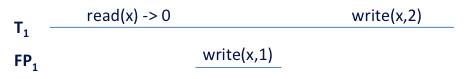
\includegraphics[width=\columnwidth]{figs/FP-why-bump}
\caption{Conflict between FP transaction $FP_1$ and regular transaction $T_1$.}
\label{fig:why-bump}
\end{figure}

In order for $T_1$ to detect this 
conflict, the version written by $FP_1$ has to exceed $T_1$'s snapshot time, i.e., $ts_r$.
To this end, we maintain a new field \emph{maxVersion} for each key, which is at least as 
high as the key's latest committed version. 
The data store needs to support two atomic operations for updating {maxVersion}.
The first is \emph{fetch-and-increment, F\&I}, which increments {maxVersion} and returns its
old value; F\&I throws an abort exception in case of wrap-around of the 
sequence number part  of  the version. 
The second operation, \emph{bump}, takes a new version  as a parameter and
sets  {maxVersion} to the maximum between this parameter and its old value.

Singleton writes  increment the version using F\&I  (line~\ref{l:fi}), and  
the post-commit of transactional writes  (line~\ref{l:txu}) bumps it 
to reflect the highest committed version.
Every transactional read bumps the key's {maxVersion}
to the reading transaction's $ts_r$  (line~\ref{l:txr}); 
transactional writes (line~\ref{l:txw}) are modified to check for conflicts, namely, 
new committed versions exceeding their $ts_r$.

In the example of Figure~\ref{fig:why-bump}, $T_1$'s read bumps $x$'s {maxVersion} to its $ts_r$, 
and so $FP_1$, which increments $x$'s maxVersion, writes $1$ with a version that exceeds $ts_r$.
Thus, $T_1$'s write  detects the conflict on $x$. 

 Note that this modification of transactional writes incurs an extra cost on
 regular (non-FP) transactions, which we quantify empirically in Section~\ref{sec:eval}.  

The \code{br} and \code{wc} operations are  similar to \code{brc} and \code{bwc}, 
respectively, except that \code{wc} uses the version read by \code{br} as its upper bound
in order to detect conflicting writes that occur between its two calls.

\subsection{Implementation and optimization}
\label{ssec:fast-impl}

Associating a maxVersion field with each key is wasteful,
both in terms of space, and in terms of the number of updates this field undergoes.
Instead, when implementing support for \sys's fast path in HBase, we aggregate the maxVersions of many keys in a single variable, 
which we call the \emph{Local Version Clock (LVC)}.
%; (similar local clocks were previously used in Mediator~\cite{mediator} and CockroachDB~\cite{cockroach}).

Our implementation \inred{uses} one LVC in each region server. 
Using a shared LVC reduces the number of updates:  
a transactional read modifies the LVC only if its $ts_r$ exceeds it. In particular, 
a transaction with multiple reads in the same region server needs to bump it only once. 

We implement the two required atomic methods - F\&I and bump on the LVC using atomic hardware operations (F\&I and CAS, respectively). 
The HBase coprocessor mechanism enforces atomic execution of the stored code blocks by holding  a lock on the affected key for the duration of the operation.
Thus, putVersion executes as an atomic block, and calls the LVC's F\&I method inside this block.
Similarly, the calls to bump from preGet and preUpdate execute inside an atomic block with the ensuing get an update, respectively. 

Note that although the coprocessor only holds a lock on the affected key, the joint update of the key and the LVC is consistent
because it uses a form of two-phase locking: when the stored procedure begins, its locks the key, then the atomic access to the LVC
effectively locks the LVC during its update; this is followed by an update of the key's record and the key's lock being released.

The LVC is kept in memory, and is not persisted. Migration of region control across region servers, which HBase performs 
to balance load and handle server crashes, must be handled by the LVC management. 
In both cases, we need to ensure that the monotonicity of the LVC associated with the %(migrated or recovered) 
region is preserved. To this end, when a region is started in a new server (following migration or recovery), 
we force the first operation accessing it
in the new server to accesses the TM to increment the global clock, and then 
bumps the local clock to the value of the global clock.
Since the LVC value can never exceed the global clock's value, this bootstrapping procedure maintains its monotonicity.



